% ===================================================================
%  Week 10 — Persian lecture notes — Feature Detection & Matching
% ===================================================================
\documentclass[12pt]{article}
% ===================================================================
%  Shared preamble for Persian lecture notes (Image Processing).
%  Compile with XeLaTeX.  Body = Persian (RTL), code/math = LTR.
% ===================================================================

\usepackage{geometry}
\geometry{a4paper,margin=2.4cm}
\usepackage{amsmath,amssymb}
\usepackage{graphicx}
\usepackage{xcolor}
\usepackage{listings}
\usepackage{tcolorbox}
\usepackage{booktabs}
\usepackage{array}
\usepackage{enumitem}
\usepackage{hyperref}
\tcbuselibrary{skins,breakable}

% ---- Persian / RTL --------------------------------------------------
\usepackage{xepersian}
\settextfont{IRNazli}
\setlatintextfont{Latin Modern Roman}
\setdigitfont{IRNazli}
% More generous leading + paragraph spacing (Persian reads better with air).
\linespread{1.5}
\setlength{\parskip}{0.7em}

% ---- Colours --------------------------------------------------------
\definecolor{coursePrimary}{HTML}{1B4965}
\definecolor{courseAccent}{HTML}{E76F51}
\definecolor{courseGood}{HTML}{2A9D8F}
\definecolor{courseBad}{HTML}{C0392B}
\definecolor{courseInfo}{HTML}{2980B9}
\definecolor{codeBg}{HTML}{F5F6FA}
\definecolor{codeKw}{HTML}{8E44AD}
\definecolor{codeStr}{HTML}{2A9D8F}
\definecolor{codeCom}{HTML}{7F8C8D}

\hypersetup{colorlinks=true,linkcolor=courseInfo,urlcolor=courseInfo,citecolor=courseInfo}

% ---- Code listings (Python built in) -------------------------------
\lstdefinestyle{course}{
  backgroundcolor=\color{codeBg},
  basicstyle=\ttfamily\small,
  keywordstyle=\color{codeKw}\bfseries,
  stringstyle=\color{codeStr},
  commentstyle=\color{codeCom}\itshape,
  numberstyle=\tiny\color{codeCom},
  numbers=left, numbersep=7pt,
  showstringspaces=false, breaklines=true,
  tabsize=4, columns=fullflexible, frame=single,
  rulecolor=\color{gray!30}, keepspaces=true, upquote=true, language=Python,
}
\lstset{style=course}
\lstdefinelanguage{bash}{
  keywords={cd,pip,python,venv,source,import}, sensitive=true,
  morecomment=[l]{\#}, morestring=[b]', morestring=[b]",
}
\newenvironment{ltrcode}{\begin{LTR}}{\end{LTR}}

% ---- Callout boxes (Persian titles) --------------------------------
\newtcolorbox{yaddasht}{colback=courseInfo!8,colframe=courseInfo,
  title={\textbf{یادداشت}},boxrule=0.6pt,right=6pt,left=6pt,breakable}
\newtcolorbox{nokte}{colback=courseAccent!10,colframe=courseAccent,
  title={\textbf{نکتهٔ کلیدی}},boxrule=0.6pt,right=6pt,left=6pt,breakable}
\newtcolorbox{hoshdar}{colback=courseBad!8,colframe=courseBad,
  title={\textbf{هشدار / دام}},boxrule=0.6pt,right=6pt,left=6pt,breakable}
\newtcolorbox{riyazi}{colback=coursePrimary!6,colframe=coursePrimary,
  title={\textbf{ریاضیات}},boxrule=0.6pt,right=6pt,left=6pt,breakable}
\newtcolorbox{tamrin}{colback=courseGood!8,colframe=courseGood,
  title={\textbf{تمرین}},boxrule=0.6pt,right=6pt,left=6pt,breakable}

% ---- Header helper --------------------------------------------------
\newcommand{\coursemeta}[2]{%
  \begin{center}
  {\large\textbf{پردازش تصویرِ کاربردی}}\\[2pt]
  {\color{coursePrimary}\rule{\linewidth}{1pt}}\\[4pt]
  {\Large\textbf{#1}}\\[3pt]
  {\small جزوهٔ درس — #2}
  \end{center}\vspace{4pt}
}


\begin{document}
\coursemeta{جلسهٔ ۱۰ — تشخیص و تطبیقِ ویژگی‌ها (Feature Detection \& Matching)}{هفتهٔ دهم}

\section*{نگاهِ کلی به این جلسه}

تا اینجا یاد گرفتیم چطور محتوای یک تصویر را توصیف کنیم: لبه‌ها، ناحیه‌ها و شکل‌ها. اما یک پرسشِ بنیادی باقی مانده است: چطور بفهمیم که یک نقطهٔ مشخص در تصویرِ اول، \emph{همان} نقطه در تصویرِ دوم است؟ اگر از یک کنتور دو عکس بگیریم — یکی صاف و یکی از زاویه و کوچک‌تر — چطور دو عکس را روی هم منطبق کنیم؟ پاسخ، مفهومِ «ویژگی» (feature) است: نقاطِ متمایز و قابلِ‌شناسایی که می‌توان آن‌ها را در تصویرهای مختلف پیدا و با هم مطابقت داد.

\begin{yaddasht}
ویژگی‌ها پایهٔ «بینایی هندسی» هستند: دوختنِ پانوراما، ردیابیِ اجسام، واقعیتِ افزوده و — برای ما — منطبق‌کردنِ عکسِ یک سند/کنتور روی الگو تا آن را صاف کنیم. این دقیقاً هستهٔ مرحلهٔ بعدیِ پروژهٔ DocScan (هفتهٔ ۱۱، تصحیحِ پرسپکتیو) است.
\end{yaddasht}

\subsection*{یک تشبیهِ ساده}

فرض کنید می‌خواهید دو عکس از یک ساختمان را — که از دو زاویهٔ متفاوت گرفته شده‌اند — روی هم منطبق کنید. اگر به دوستی بگویید «این گوشهٔ پنجرهٔ سومِ طبقهٔ دو» را در هر دو عکس پیدا کند، او به‌راحتی این کار را می‌کند، چون آن گوشه یک نشانهٔ متمایز است. اما اگر بگویید «این نقطه از دیوارِ یک‌دست» را پیدا کن، ناتوان می‌ماند، چون همهٔ نقاطِ دیوار شبیهِ هم‌اند. کامپیوتر هم دقیقاً همین‌طور است: به نقاطِ متمایز (ویژگی‌ها) و یک «توضیحِ» فشرده از هر نقطه (توصیف‌گر) نیاز دارد تا بتواند تناظر برقرار کند. کلِ این جلسه دربارهٔ همین دو چیز است: چطور نقاطِ متمایز را پیدا کنیم، و چطور آن‌ها را طوری توصیف کنیم که با وجودِ چرخش و تغییرِ اندازه بازشناختنی بمانند.

\section{ویژگیِ خوب چیست؟}

هر نقطه‌ای برای تطبیق مناسب نیست. یک نقطه در وسطِ یک دیوارِ صاف و یک‌دست، هیچ نشانهٔ متمایزی ندارد؛ اگر کمی جابه‌جا شویم، منظره فرقی نمی‌کند، پس نمی‌توانیم دوباره «همان» نقطه را پیدا کنیم. یک ویژگیِ خوب سه خاصیت دارد:

\begin{itemize}
  \item \textbf{متمایز (Distinctive):} با محیطِ اطرافش فرق دارد، پس دوباره قابلِ پیدا‌شدن است.
  \item \textbf{تکرارپذیر (Repeatable):} همان نقطهٔ فیزیکی در تصویرهای مختلف (زاویه یا نورِ متفاوت) باز هم شناسایی می‌شود.
  \item \textbf{محلی (Local):} با یک وصلهٔ کوچک توصیف می‌شود، پس در برابرِ پوشیده‌شدنِ بخشی از تصویر مقاوم است.
\end{itemize}

\subsection{چرا گوشه؟}

سه حالت را در نظر بگیرید و تصور کنید یک پنجرهٔ کوچک را روی تصویر کمی جابه‌جا می‌کنیم:

\begin{itemize}
  \item \textbf{ناحیهٔ صاف:} جابه‌جایی در هر جهت، منظره را تغییر نمی‌دهد $\rightarrow$ هیچ مکان‌یابی‌ای ممکن نیست.
  \item \textbf{لبه:} جابه‌جایی \emph{در امتدادِ} لبه تغییری ایجاد نمی‌کند $\rightarrow$ ابهامِ یک‌بُعدی (نمی‌دانیم کجای لبه هستیم).
  \item \textbf{گوشه:} جابه‌جایی در \emph{هر} جهت منظره را تغییر می‌دهد $\rightarrow$ نقطه در دو بُعد کاملاً مشخص است.
\end{itemize}

\begin{nokte}
به همین دلیل «گوشه» کلاسیک‌ترین ویژگیِ خوب است: تنها جایی که موقعیتش را به‌طورِ یکتا در صفحه می‌خ‌میخکوبد. آشکارسازِ \textbf{هریس} (Harris) دقیقاً همین را می‌سنجد: میزانِ تغییرِ شدت در همهٔ جهت‌ها.
\end{nokte}

\subsection{ماتریسِ ساختار (Structure Matrix)}

هریس چطور کار می‌کند؟ درونِ یک پنجرهٔ کوچک، گرادیان‌های تصویر $(I_x, I_y)$ را نگاه می‌کنیم و ماتریسِ $۲\times۲$ زیر را می‌سازیم:

\begin{riyazi}
\[
M = \sum_{\text{پنجره}} \begin{pmatrix} I_x^2 & I_x I_y \\ I_x I_y & I_y^2 \end{pmatrix}
\]
دو مقدارِ ویژهٔ این ماتریس، $\lambda_1$ و $\lambda_2$، می‌گویند وصله در دو جهتِ اصلی چقدر تغییر می‌کند:
\begin{itemize}
  \item هر دو کوچک $\rightarrow$ ناحیهٔ صاف.
  \item یکی بزرگ، یکی کوچک $\rightarrow$ لبه.
  \item هر دو بزرگ $\rightarrow$ \textbf{گوشه}.
\end{itemize}
برای پرهیز از محاسبهٔ مستقیمِ مقادیرِ ویژه، هریس امتیازِ $R=\lambda_1\lambda_2 - k(\lambda_1+\lambda_2)^2 = \det(M) - k\,\mathrm{tr}(M)^2$ را حساب می‌کند ($k\approx0.04$).
\end{riyazi}

در شکلِ زیر، آشکارسازِ هریس را روی یک خودروی واقعی از مجموعه‌دادهٔ شما اجرا کرده‌ایم. نقاطِ قرمز، گوشه‌های شناسایی‌شده هستند:

\begin{center}
  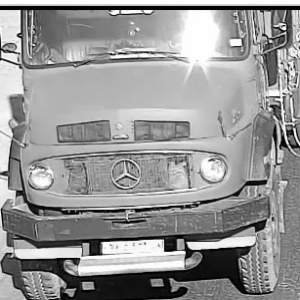
\includegraphics[width=0.44\linewidth]{../assets/gray.png}\hfill
  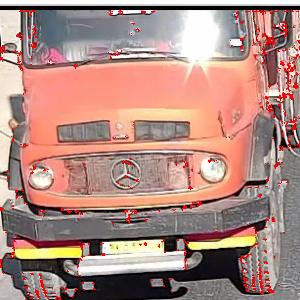
\includegraphics[width=0.44\linewidth]{../assets/harris.png}\\
  {\small چپ: تصویرِ خاکستری \quad راست: گوشه‌های هریس (قرمز) روی محل‌های متمایز}
\end{center}

می‌بینید که گوشه‌ها روی محل‌های متمایز (چراغ‌ها، لبه‌های قطعات، محلِ اتصالِ اجزا) می‌نشینند — همان نقاطی که در عکسِ دیگری از همان خودرو هم قابلِ پیدا‌شدن‌اند.

\subsection{آشکارسازِ FAST، گام‌به‌گام}

هریس دقیق است اما کُند؛ برای کاربردهای بی‌درنگ (ویدیو) به چیزِ سریع‌تری نیاز داریم. \textbf{FAST} (Features from Accelerated Segment Test) یک آزمونِ بسیار ساده و سریع دارد:

\begin{enumerate}
  \item یک دایره از ۱۶ پیکسل را دورِ پیکسلِ موردِنظر $p$ در نظر بگیر.
  \item اگر دستِ‌کم ۱۲ پیکسلِ پیوسته روی این دایره همگی \emph{روشن‌تر} از $p$ (به‌اندازهٔ یک آستانه $t$) یا همگی \emph{تیره‌تر} باشند، آن‌گاه $p$ یک گوشه است.
  \item برای سرعت، ابتدا فقط ۴ پیکسلِ بالا/پایین/چپ/راست بررسی می‌شوند؛ اگر شرط برقرار نباشد، پیکسل فوراً رد می‌شود.
\end{enumerate}

\begin{nokte}
همین آزمونِ ساده، FAST را ده‌ها برابر سریع‌تر از هریس می‌کند و به همین دلیل هستهٔ آشکارسازِ ORB است. بهایش این است که FAST به‌تنهایی مقیاس و جهت را نمی‌دهد؛ ORB این‌ها را با هرمِ تصویر و محاسبهٔ جهتِ گشتاور اضافه می‌کند.
\end{nokte}

\section{از نقطهٔ کلیدی تا توصیف‌گر}

پیداکردنِ \emph{محلِ} ویژگی (نقطهٔ کلیدی یا keypoint) تنها گامِ اول است. گامِ دوم این است که \emph{ظاهرِ} آن نقطه را چطور توصیف کنیم تا بتوانیم آن را در تصویرِ دیگر بازبشناسیم. این کار با \textbf{توصیف‌گر} (descriptor) انجام می‌شود: برداری که وصلهٔ اطرافِ نقطهٔ کلیدی را خلاصه می‌کند.

\begin{yaddasht}
یک توصیف‌گرِ خوب باید \textbf{ناوردا} (invariant) باشد: مقدارش با چرخش، تغییرِ اندازه و تغییرِ روشنایی ثابت بماند. اگر توصیف‌گرِ یک نقطه در عکسِ صاف و عکسِ چرخیده یکسان باشد، می‌توانیم آن دو را مطابقت دهیم.
\end{yaddasht}

معروف‌ترین توصیف‌گرِ کلاسیک، \textbf{SIFT} است: یک بردارِ ۱۲۸‌بُعدی از هیستوگرام‌های جهتِ گرادیان، که در برابرِ چرخش، مقیاس و روشنایی بسیار مقاوم است. توصیف‌گرِ عملی‌ترِ ما \textbf{ORB} است.

\subsection{ORB روی خودروی واقعی}

ORB ترکیبی است از نقاطِ کلیدیِ FAST به‌علاوهٔ توصیف‌گرِ باینریِ BRIEF که آگاه‌به‌چرخش شده است. رایگان و سریع است. در شکلِ زیر، ۳۸۰ نقطهٔ کلیدیِ ORB روی همان خودرو را می‌بینید؛ هر دایره یک نقطهٔ کلیدی با اندازه (مقیاس) و جهت است:

\begin{center}
  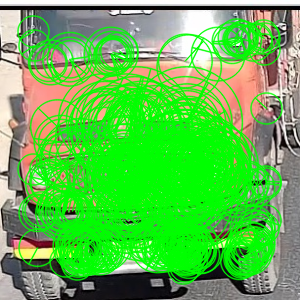
\includegraphics[width=0.5\linewidth]{../assets/orb_keypoints.png}\\
  {\small ۳۸۰ نقطهٔ کلیدیِ ORB؛ هر دایره یک ویژگیِ متمایز با توصیف‌گرِ باینری است}
\end{center}

\subsection{هریس در برابرِ شی-توماسی}

شاید بپرسید چرا چند آشکارسازِ گوشه داریم. تفاوت در «امتیازی» است که هر کدام برای گوشه‌بودن حساب می‌کند:

\begin{itemize}
  \item \textbf{هریس} از فرمولِ $R=\det(M)-k\,\mathrm{tr}(M)^2$ استفاده می‌کند که به پارامترِ حساسِ $k$ نیاز دارد.
  \item \textbf{شی-توماسی} (تابعِ \texttt{goodFeaturesToTrack}) به‌جای آن مستقیماً \emph{کوچک‌ترین} مقدارِ ویژه $\min(\lambda_1,\lambda_2)$ را امتیاز می‌دهد. منطقش این است: یک گوشهٔ خوب باید در \emph{هر دو} جهت تغییرِ قوی داشته باشد، پس ضعیف‌ترین جهت را می‌سنجیم.
\end{itemize}

\begin{nokte}
شی-توماسی در عمل برای \textbf{ردیابی} (دنبال‌کردنِ نقاط در ویدیو) پایدارتر است و به همین دلیل در الگوریتم‌های ردیابیِ نوریِ (optical flow) کلاسیک محبوب است. برای ما هر دو نشان می‌دهند که «آشکارسازی» یک مسئلهٔ طراحیِ امتیاز است، نه یک جوابِ یکتا.
\end{nokte}

\subsection{مقایسهٔ توصیف‌گرها}

\begin{center}
\begin{tabular}{@{}lll@{}}
\hline
\textbf{توصیف‌گر} & \textbf{نوع} & \textbf{ویژگی} \\
\hline
SIFT & اعشاری ۱۲۸‌بُعدی & بسیار مقاوم؛ استانداردِ طلایی \\
SURF & اعشاری & شبیهِ SIFT اما سریع‌تر (دارای ثبتِ اختراع) \\
ORB & باینری ۲۵۶‌بیتی & رایگان، سریع، عالی برای بی‌درنگ \\
BRIEF & باینری & سریع اما به‌تنهایی ناوردا‌به‌چرخش نیست \\
\hline
\end{tabular}
\end{center}

\begin{nokte}
پیش‌فرضِ عملیِ ما ORB است: رایگان، سریع و به‌قدرِ کافی خوب. وقتی به بیشترین مقاومت نیاز داشتید (مثلاً تغییرِ ظاهرِ شدید)، سراغِ SIFT بروید.
\end{nokte}

\section{تطبیقِ توصیف‌گرها میانِ تصویرها}

حالا که برای هر نقطهٔ کلیدی یک توصیف‌گر داریم، تطبیق ساده است: برای هر توصیف‌گر در تصویرِ A، \emph{نزدیک‌ترین} توصیف‌گر در تصویرِ B را (بر اساسِ فاصله) پیدا می‌کنیم.

\begin{itemize}
  \item برای توصیف‌گرهای اعشاری (SIFT): فاصلهٔ اقلیدسی.
  \item برای توصیف‌گرهای باینری (ORB): فاصلهٔ \textbf{همینگ} — تعدادِ بیت‌های متفاوت، که با یک XOR و شمارشِ بیت بسیار سریع محاسبه می‌شود.
  \item روشِ \textbf{جست‌وجوی فراگیر} (Brute-force) همهٔ جفت‌ها را مقایسه می‌کند؛ \textbf{FLANN} برای مجموعه‌های بزرگ این کار را تقریبی و سریع انجام می‌دهد.
\end{itemize}

در شکلِ زیر، همان خودرو را چرخانده و کوچک کرده‌ایم (چرخشِ ۳۰ درجه، مقیاسِ ۰٫۸) و ویژگی‌های ORB را بینِ نسخهٔ اصلی و نسخهٔ تغییریافته مطابقت داده‌ایم. خط‌ها نقاطِ فیزیکیِ یکسان را به هم وصل می‌کنند:

\begin{center}
  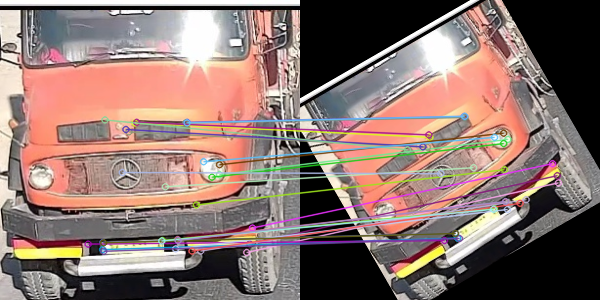
\includegraphics[width=0.9\linewidth]{../assets/matches.png}\\
  {\small تطبیقِ ORB بینِ خودرو و نسخهٔ چرخیده/کوچک‌شدهٔ آن — ناوردایی در عمل، روی دادهٔ واقعی}
\end{center}

این تصویر قلبِ درس است: با وجودِ چرخش و تغییرِ اندازه، ویژگی‌ها هنوز درست مطابقت می‌خورند. \emph{این} همان چیزی است که به آن «ناوردایی» می‌گوییم.

\subsection{یک مثالِ عددیِ فاصلهٔ همینگ}

فرض کنید دو توصیف‌گرِ باینریِ ۸‌بیتی داریم (توصیف‌گرِ واقعیِ ORB ۲۵۶‌بیتی است، اما اصل یکسان است):

\begin{riyazi}
\begin{align*}
d_1 &= 1\,0\,1\,1\,0\,0\,1\,0 \\
d_2 &= 1\,0\,0\,1\,0\,1\,1\,0 \\
d_1 \oplus d_2 &= 0\,0\,1\,0\,0\,1\,0\,0
\end{align*}
تعدادِ بیت‌های ۱ در حاصلِ XOR برابرِ $۲$ است، پس فاصلهٔ همینگ $=۲$. یعنی این دو توصیف‌گر تنها در ۲ بیت از ۸ بیت تفاوت دارند — بسیار شبیه‌اند و احتمالاً یک تطبیقِ درست‌اند.
\end{riyazi}

چون این محاسبه فقط یک XOR و یک شمارشِ بیت (popcount) است، پردازنده‌های امروزی آن را در یک دستور انجام می‌دهند؛ به همین دلیل تطبیقِ توصیف‌گرهای باینری بسیار سریع است.

\subsection{کنار‌گذاشتنِ تطبیق‌های بد}

بسیاری از تطبیق‌های نزدیک‌ترین‌همسایه غلط‌اند. باید فیلترشان کنیم:

\begin{itemize}
  \item \textbf{آزمونِ نسبت (Ratio Test) — لُوو:} یک تطبیق را فقط وقتی نگه می‌داریم که بهترین همسایه به‌طورِ محسوسی از دومین‌همسایه نزدیک‌تر باشد (مثلاً فاصلهٔ اول $<0.75\times$ فاصلهٔ دوم). اگر دو همسایه تقریباً هم‌فاصله باشند، تطبیق مبهم است و دور انداخته می‌شود.
  \item \textbf{بررسیِ متقابل (Cross-check):} فقط تطبیق‌هایی را نگه می‌داریم که در هر دو جهت نزدیک‌ترین همسایه باشند.
  \item \textbf{RANSAC (هفتهٔ ۱۱):} برون‌داده‌های هندسی را با برازشِ یک تبدیل کنار می‌گذارد.
\end{itemize}

\begin{hoshdar}
تطبیق‌های خام پُرنویز‌اند. بدونِ آزمونِ نسبت یا RANSAC، حتی چند تطبیقِ غلط می‌تواند کلِ فرآیندِ انطباق را خراب کند. همیشه فیلتر کنید.
\end{hoshdar}

\subsection{چرا آستانهٔ ۰٫۷۵ در آزمونِ نسبت؟}

دیوید لُوو (مبتکرِ SIFT) با آزمایش روی هزاران تطبیق نشان داد که اگر نسبتِ فاصلهٔ نزدیک‌ترین‌همسایه به دومین‌نزدیک‌ترین را رسم کنیم، تطبیق‌های \emph{درست} تقریباً همیشه نسبتِ کوچکی دارند (اولی خیلی نزدیک‌تر است)، در حالی که تطبیق‌های \emph{غلط} نسبتی نزدیک به ۱ دارند (هر دو همسایه تصادفی و تقریباً هم‌فاصله‌اند). آستانهٔ $۰٫۷۵$ حدودِ ۹۰٪ تطبیق‌های غلط را حذف می‌کند و تنها حدودِ ۵٪ تطبیق‌های درست را از دست می‌دهد — معاملهٔ بسیار خوبی.

\begin{yaddasht}
نکتهٔ عملی: آزمونِ نسبت به \texttt{knnMatch} با $k=۲$ نیاز دارد (دو همسایهٔ نزدیک برای هر نقطه)، نه \texttt{match} با بررسیِ متقابل. این دو راهبردِ فیلترکردن‌اند و معمولاً یکی را انتخاب می‌کنید.
\end{yaddasht}

\section{ناوردایی به مقیاس: هرمِ تصویر}

چطور یک ویژگی را در هر اندازه‌ای پیدا کنیم؟ با ساختنِ \textbf{هرمِ تصویر} (image pyramid): مجموعه‌ای از نسخه‌های به‌تدریج کوچک‌ترِ همان تصویر. ویژگی‌ها را در هر مقیاس آشکار می‌کنیم؛ مقیاسی که در آن ویژگی قوی‌ترین پاسخ را می‌دهد، «مقیاسِ مشخصهٔ» آن ویژگی است. به همین ترتیب SIFT و ORB می‌توانند یک الگوی کوچک را با یک عکسِ بزرگ مطابقت دهند.

\begin{riyazi}
برای برآوردِ یک \textbf{هوموگرافی} (تبدیلِ پرسپکتیو، هفتهٔ ۱۱) به دستِ‌کم $۴$ تطبیقِ خوب نیاز است. در عمل ده‌ها تطبیق جمع می‌کنیم و می‌گذاریم RANSAC یک زیرمجموعهٔ سازگارِ ۴‌تایی (یا بیشتر) را انتخاب کند. هرچه تطبیق‌های خوبِ بیشتری داشته باشیم، تبدیلِ برآوردشده پایدارتر و دقیق‌تر است.
\end{riyazi}

\section{راهبردهای تطبیق در یک نگاه}

سه راهبردِ رایج برای تطبیق و فیلترکردن وجود دارد؛ انتخابِ درست به کاربردِ شما بستگی دارد:

\begin{center}
\begin{tabular}{@{}lll@{}}
\hline
\textbf{راهبرد} & \textbf{چگونه} & \textbf{کِی استفاده} \\
\hline
بررسیِ متقابل & \texttt{BFMatcher(crossCheck=True)} & ساده، سریع، تطبیقِ یک‌به‌یک \\
آزمونِ نسبت & \texttt{knnMatch(k=2)} + آستانه & دقیق‌ترین فیلتر؛ توصیهٔ لُوو \\
FLANN & درختِ تقریبی & مجموعه‌های خیلی بزرگِ ویژگی \\
\hline
\end{tabular}
\end{center}

\begin{hoshdar}
یک اشتباهِ رایج: استفادهٔ هم‌زمان از \texttt{crossCheck=True} و \texttt{knnMatch}. این دو با هم ناسازگارند؛ \texttt{knnMatch} برای هر نقطه چند همسایه می‌خواهد، اما \texttt{crossCheck} فقط یک تطبیقِ متقابل برمی‌گرداند. یکی را انتخاب کنید.
\end{hoshdar}

\subsection{اشتباه‌های رایجِ دانشجویان}

\begin{itemize}
  \item \textbf{فراموشیِ تبدیل به خاکستری:} آشکارسازها روی تصویرِ تک‌کاناله کار می‌کنند؛ دادنِ تصویرِ رنگی گاهی خطا یا نتیجهٔ ضعیف می‌دهد.
  \item \textbf{نگه‌داشتنِ همهٔ تطبیق‌ها:} بدونِ فیلتر، تطبیق‌های غلط کلِ انطباق را خراب می‌کنند. همیشه فیلتر کنید.
  \item \textbf{انتظارِ ویژگی روی سطحِ صاف:} روی یک برگهٔ سفیدِ بی‌بافت، ORB نقاطِ کمی پیدا می‌کند؛ باید به لبه‌ها و بافتِ کادر تکیه کرد.
  \item \textbf{مقایسهٔ توصیف‌گرهای ناهم‌جنس:} فاصلهٔ همینگ فقط برای توصیف‌گرهای باینری (ORB/BRIEF) است؛ برای SIFT از \texttt{NORM\_L2} استفاده کنید.
\end{itemize}

\section{کاربردها}

\begin{itemize}
  \item \textbf{دوختنِ تصویر (پانوراما):} ویژگی‌ها را مطابقت بده، تبدیل را پیدا کن، تصویرها را ادغام کن.
  \item \textbf{شناساییِ شیء:} ویژگی‌های یک الگو را با صحنه مطابقت بده.
  \item \textbf{ردیابی، SLAM و واقعیتِ افزوده:} ویژگی‌ها را در طولِ ویدیو دنبال کن تا حرکت را برآورد کنی.
  \item \textbf{DocScan:} صفحه/الگو را مطابقت بده تا آن را منطبق و صاف کنی (هفتهٔ ۱۱).
\end{itemize}

\subsection{ویژگی‌های کلاسیک در برابرِ عمیق}

ویژگی‌های کلاسیک (SIFT/ORB) دست‌طراحی، قابلِ‌تفسیر و بدونِ نیاز به آموزش‌اند و هنوز برای مسائلِ هندسی عالی عمل می‌کنند. توصیف‌گرهای عمیق (مثلِ SuperPoint) در تغییرِ ظاهرِ شدید بهتر عمل می‌کنند اما به آموزش نیاز دارند. برای انطباق و هندسه، ویژگی‌های کلاسیک همچنان انتخابی قوی و عملی هستند.

\begin{nokte}
جمع‌بندیِ مفهومی: ویژگی راهی است که کامپیوتر بگوید «این نقطه در اینجا، همان نقطه در آنجاست». همین توانایی، بنیادِ همهٔ بینایی هندسی است.
\end{nokte}

\subsection{سناریوی DocScan: منطبق‌کردنِ عکسِ کنتور روی الگو}

بیایید کاربردِ مستقیمِ این جلسه در پروژه را قدم‌به‌قدم ببینیم. فرض کنید یک «الگو» (تصویرِ تمیزِ روبه‌رو از صفحهٔ کنتور) داریم و کاربر با موبایل عکسی کج و از زاویه گرفته است:

\begin{enumerate}
  \item روی هر دو تصویر ویژگی‌های ORB را آشکار و توصیف می‌کنیم.
  \item توصیف‌گرها را با فاصلهٔ همینگ مطابقت می‌دهیم و با آزمونِ نسبت فیلتر می‌کنیم؛ چند ده تطبیقِ خوب می‌ماند.
  \item این تطبیق‌ها می‌گویند «گوشهٔ بالا‌چپِ کادرِ کنتور در الگو، در عکس کجاست»، و همین‌طور برای بقیهٔ نقاط.
  \item هفتهٔ آینده با \texttt{findHomography} یک تبدیلِ پرسپکتیو از این تطبیق‌ها برآورد می‌کنیم و با \texttt{warpPerspective} عکسِ کج را به نمای روبه‌رو و صاف تبدیل می‌کنیم — آمادهٔ خواندنِ ارقام.
\end{enumerate}

\begin{nokte}
پس ویژگی‌ها «چسبِ هندسیِ» DocScan‌اند: بدونِ آن‌ها نمی‌دانیم کدام نقطهٔ عکس با کدام نقطهٔ الگو متناظر است، و بدونِ این تناظر نمی‌توان تصویر را صاف کرد.
\end{nokte}

\section{کد: از آشکارسازی تا تطبیق}

\begin{ltrcode}
\begin{lstlisting}[language=Python]
import cv2
img1 = cv2.imread('meter.jpg', 0)
img2 = cv2.imread('meter_tilted.jpg', 0)

orb = cv2.ORB_create(500)
kp1, des1 = orb.detectAndCompute(img1, None)
kp2, des2 = orb.detectAndCompute(img2, None)

# match with cross-check
bf = cv2.BFMatcher(cv2.NORM_HAMMING, crossCheck=True)
matches = sorted(bf.match(des1, des2), key=lambda m: m.distance)

# draw the best 30
out = cv2.drawMatches(img1, kp1, img2, kp2, matches[:30], None)
cv2.imwrite('matches.png', out)
# next week: cv2.findHomography(pts1, pts2, cv2.RANSAC) to align
\end{lstlisting}
\end{ltrcode}

الگوی همیشگی: آشکارسازی $\rightarrow$ توصیف $\rightarrow$ تطبیق $\rightarrow$ (هفتهٔ ۱۱) برآوردِ تبدیل.

\section{چطور کیفیتِ ویژگی‌ها را بسنجیم؟}

وقتی روی دادهٔ خودتان کار می‌کنید، از کجا بدانید آشکارسازتان خوب عمل می‌کند؟ دو معیارِ عملی:

\begin{itemize}
  \item \textbf{تکرارپذیری (Repeatability):} تصویر را کمی بچرخانید یا مقیاسش را عوض کنید؛ چه کسری از نقاطِ کلیدی دوباره (تقریباً در همان محلِ فیزیکی) پیدا می‌شوند؟ هرچه بیشتر، بهتر.
  \item \textbf{نرخِ تطبیقِ درست (Precision):} از تطبیق‌هایی که الگوریتم برمی‌گرداند، چه کسری واقعاً درست‌اند؟ این را می‌توان با دانستنِ تبدیلِ واقعی (مثلاً وقتی خودتان تصویر را چرخانده‌اید) سنجید.
\end{itemize}

\begin{riyazi}
در مثالِ خودروی این جلسه، ما تبدیل را \emph{می‌دانستیم} (چرخشِ ۳۰ درجه، مقیاسِ ۰٫۸)، پس می‌توانستیم بررسی کنیم که آیا هر تطبیق با این تبدیل سازگار است یا نه. همین ایده، هستهٔ RANSAC در هفتهٔ آینده است: تبدیل را \emph{نمی‌دانیم}، پس آن را از خودِ تطبیق‌ها حدس می‌زنیم و تطبیق‌های ناسازگار را دور می‌ریزیم.
\end{riyazi}

\begin{yaddasht}
درسِ مهندسی: هر جزءِ سامانه را با یک معیارِ کمی بسنجید. «به‌نظر خوب می‌آید» کافی نیست؛ «۹۲٪ تطبیق‌ها درست‌اند» قابلِ اتکا و قابلِ بهبود است.
\end{yaddasht}

\section{کدِ کامل‌تر: آزمونِ نسبت}

\begin{ltrcode}
\begin{lstlisting}[language=Python]
# ratio test (Lowe) - the recommended filter
bf = cv2.BFMatcher(cv2.NORM_HAMMING)   # no crossCheck with knnMatch
knn = bf.knnMatch(des1, des2, k=2)     # 2 nearest neighbours each
good = []
for m, n in knn:
    if m.distance < 0.75 * n.distance: # best clearly closer than 2nd
        good.append(m)
print(f"kept {len(good)} of {len(knn)} matches")
\end{lstlisting}
\end{ltrcode}

\section{تمرینِ کلاسی و پاسخ}

\begin{tamrin}
۱) چرا یک گوشه ویژگیِ بهتری از یک نقطه در وسطِ دیوارِ صاف است؟\\
۲) یک الگوی پلاک را با عکسی که از زاویه و نصفِ اندازه گرفته شده مطابقت می‌دهید؛ کدام خاصیتِ توصیف‌گر این کار را ممکن می‌کند؟\\
۳) پس از تطبیق، چند خط به‌وضوح غلط‌اند (درهم‌رفته). چطور حذفشان می‌کنید؟
\end{tamrin}

\textbf{پاسخ‌ها:} (۱) گوشه در \emph{همهٔ} جهت‌ها تغییر می‌کند، پس به‌طورِ یکتا مکان‌یابی می‌شود؛ نقطهٔ صاف مبهم است. (۲) ناوردایی به مقیاس و چرخش — توصیف‌گر با وجودِ تغییرِ اندازه و زاویه یکسان می‌ماند. (۳) آزمونِ نسبت و بررسیِ متقابل بیشترشان را حذف می‌کنند؛ RANSAC (هفتهٔ ۱۱) برون‌داده‌های هندسی را با برازشِ یک تبدیل کنار می‌گذارد.

\section{زمینهٔ تاریخی و پیوند با ادامهٔ درس}

آشکارسازِ گوشهٔ هریس در سالِ ۱۹۸۸ معرفی شد و SIFT در سالِ ۱۹۹۹ توسطِ دیوید لُوو — این‌ها انقلابی در بینایی ماشین بودند، چون برای اولین بار امکانِ تطبیقِ قابلِ‌اعتماد بینِ تصویرهای بسیار متفاوت را فراهم کردند. تا پیش از دورانِ یادگیریِ عمیق (حدودِ ۲۰۱۲)، تقریباً هر سامانهٔ شناساییِ شیء بر پایهٔ همین ویژگی‌های دست‌طراحی بنا شده بود. امروز هم برای مسائلِ \emph{هندسی} (انطباق، دوخت، بازسازیِ سه‌بُعدی) این ویژگی‌ها همچنان انتخابِ اول‌اند، چون سریع، قابلِ‌تفسیر و بی‌نیاز از آموزش‌اند.

\begin{yaddasht}
نقشهٔ راهِ پروژه: هفتهٔ ۹ کانتورِ بیرونیِ سند را به ۴ گوشه تقریب زدیم؛ این هفته یاد گرفتیم نقاطِ متناظر را بینِ دو تصویر پیدا کنیم؛ هفتهٔ ۱۱ از این تناظرها یک تبدیلِ پرسپکتیو می‌سازیم و تصویر را صاف می‌کنیم؛ و در هفته‌های ۱۲ تا ۱۴ ارقامِ صاف‌شده را با یادگیریِ ماشین و شبکه‌های عصبی می‌خوانیم. هر هفته یک حلقه از همین زنجیره است.
\end{yaddasht}

هم‌چنین توجه کنید که ویژگی‌ها پلی به سمتِ یادگیریِ ماشین هم هستند: در هفتهٔ ۱۲ خواهیم دید که می‌توان از توصیف‌گرها به‌عنوانِ «ویژگیِ ورودی» برای یک طبقه‌بند استفاده کرد — درست همان‌طور که یک انسان اجسام را با نشانه‌های متمایزشان تشخیص می‌دهد.

\section{جمع‌بندی}

در این جلسه یاد گرفتیم ویژگیِ خوب چیست (متمایز، تکرارپذیر، محلی) و چرا گوشه‌ها انتخابِ کلاسیک‌اند؛ گوشه‌ها را با هریس/FAST آشکار کردیم و توصیف‌گر را با ORB/SIFT ساختیم؛ توصیف‌گرها را مطابقت دادیم و تطبیق‌های بد را با آزمونِ نسبت و بررسیِ متقابل حذف کردیم؛ و دیدیم ناوردایی به مقیاس و چرخش چطور روی دادهٔ واقعی کار می‌کند. هفتهٔ آینده از همین تطبیق‌ها برای برآوردِ هوموگرافی و صاف‌کردنِ عکسِ سند/کنتور در DocScan استفاده می‌کنیم.

\end{document}
